\chapter{Методика информационного взаимодействия компонентов модульного технологического оборудования}\label{ch:ch3}

\section{Подсистема управления модульным оборудованием}\label{sec:ch3/sec1}

Современные системы управления технологическим оборудованием сложны и надежны. Каждый их элемент элемент представляет собой черный ящик с жесткой иерархической архитектурой. Все в таких системах ориентировано на обеспечение качества, надежности и отказоустойчивости. Инерция таких систем вынуждает разработчиков SCADA использовать монолитную архитектуру, поскольку оборудование с распределенным управлением не может быть легко добавлено в распределенную производственную среду.

Следовательно, акцент делается на концепции интеграции. Другими словами, разработчики сосредоточились на объединении разнородных компонентов в одну производственную систему вместо использования концепции взаимодействия. Концепция взаимодействия влечет за собой создание открытого интерфейса, который позволяет компонентам оставаться в автономном состоянии с возможностью обмена данными.

Рассматриваемое модульное оборудование требует переосмысления данного подхода и создания системы управления, которая состоит из взаимозаменяемых строительных блоков с описанной унификацией ввода и вывода. При создании новой конфигурации оборудования (установке модуля/модулей на шасси) должна автоматически изменяться и подсистема управления получившимся оборудованием. Следовательно устройство ЧПУ должно знать о каждом возможном модуле заранее, то есть снова будет получена монолитная система с иерархическим управлением.

Следовательно, необходимо выделить основную часть архитектуры и определить спецификации в отношении протокола связи, а также правила создания новых программных и аппаратных модулей, которые могут быть динамически подключены к системе. Впоследствии в основную часть войдет алгоритм управления двигателями координатного шасси, а остальная часть будет внешними компонентами.

Такой подход дает возможность полностью изменить парадигму среды управления производством. К сожалению, не все так просто. Система ЧПУ - это не только алгоритм управления, но и база данных, пользовательский интерфейс и компонент связи с физической средой (также известный как «встроенные системы» и «микроконтроллеры»). Для реализации такой системы требуется системный подход, и авторы предлагают использовать шаблон архитектуры микросервисов~\cite{microservices2017indin}.

\section{Сетевая архитектура модульного оборудования}\label{sec:ch3/sec2}

Основная особенность модульного промышленного оборудования заключается в возможности быстрой переналадки любой единицы оборудования при смене технологического процесса. Переналадка осуществляется за счет смены обрабатывающих головок и внешних модулей.  Это достигается посредством максимальной автономности каждой головки или модуля. Все они обладают собственными алгоритмами функционирования, а также набором датчиков и исполнительных устройств. Все головки и модули могут общаться друг с другом по единому протоколу, при этом набор команд и данных сведен к минимуму, все команды строго регламентированы.

Основным модулем является многокоординатное шасси, которое осуществляет перемещение обрабатывающих головок в пространстве. Естественно, с точки зрения управления такая система не может быть полностью децентрализованной "--- с каждой единицей оборудования связана ее виртуальная диспетчер (<<цифровой двойник>>), который является моделью оборудования и осуществляет координацию модулей, головок и шасси. Именно наличие диспетчера позволяет осуществить быструю переналадку оборудования. Все головки и модули настроены одинаково, все они знают свои возможности и протокол взаимодействия, поэтому при физическом подключении находят в сети своего диспетчера, регистрируют свои сервисы, после чего сразу готовы к работе.

Данная концепция отлично работает, если представить, что у нас есть только одна единица оборудования, однако это не так. ИКФС может состоять из многих сотен и тысяч устройств, причем подавляющее большинство этих устройств является именно технологическим оборудованием. При этом, как уже было сказано выше, каждая единица оборудования, каждая обрабатывающая головка, каждый модуль и каждый датчик подключены к единой децентрализованной mesh-сети, т.\:к. являются частями одной ИКФС.

Здесь сразу прослеживается проблема: если все модули находятся к децентрализованной сети и имеют возможность найти своего диспетчера, то как они могут определить, что именно этот диспетчер физически подключен к данному модулю. Естественное решение: возложить эту обязанность на оператора. Однако это сломает принцип zero config, то есть оператор должен думать только о технологическом процессе, а не о конфигурации/переконфигурации оборудования. Здесь можно привести аналогию с обычным универсальным оборудованием. Рабочий, производящий операции, например, на токарном станке, не должен задумываться об информационной совместимости инструмента и станка. Ему достаточно физической совместимости. Например, резец физически помещается в резцедержатель. Именно подобной простоты переналадки мы и хотим добиться в своей работе, только не для <<глупого>> универсального оборудования, а для <<умного>>, интегрированного в ИКФС.

Из всего вышесказанного можно сделать вывод о том, что организация ячеистой сети ИКФС, в которой используется модульное оборудование, не является тривиальной задачей. Поэтому оставшаяся часть раздела будет посвящена вопросам развертывания тестовой сети OpenThread, описанию общей архитектуры ИКФС, построенное на ее основе, а также принципов работы модульного оборудования, входящего в ИКФС.


Как уже было отмечено в предыдущем разделе по совокупности достоинств и недостатков в качестве опорной сети ИКФС была выбрана технология OpenThread. Данный протокол беспроводной передачи данных является a BSD licensed open-source implementation of сетевого протокола Thread изначально разработанного компанией Google Nest. Отличительной особенностью OpenThread является максимальная переносимость, при этом в соответствии со спецификацией  могут быть реализованы различные designs, как чисто аппаратные, так и программно-аппаратные. Подобная гибкость позволяет сначала создать структуру опорной сети с применением технологий виртуализации, протестировать и отладить ее, а затем перенести на физические устройства.

Для развертывания виртуальной сети был использован набор отладки, находящийся в репозитории OpenThread (ссылка). В частности, 	использовалась сборка сетевого клиента под архитектуру x86 с эмуляцией радиомодуля посредством сетевой карты с передачей сообщений по протоколу UDP. Первостепенными задачами стали построение простейшей сети и отработка на ее примере алгоритма взаимодействия узлов. В целях упрощения задачи первоначальная структура сети состояла из трех независимых узлов. Каждый узел сети развертывается единообразно, что позволило автоматизировать этот процесс в виртуальном окружении.
В соответствие со спецификацией протокола существует два вида узлов: 

\begin{enumerate}
	\item Router, который никогда не выключает приемопередатчик, участвует в передаче пакетов по сети, а также является узлом обеспечения безопасности для всех вновь подключающихся устройств.
	\item End Device, который преимущественно взаимодействует только со своим роутером, не осуществляет передачу данных по сети и может выключать свой приемопередатчик для экономии энергии.
\end{enumerate}

В дополнение к этому все устройства в mesh-сети OpenThread могут быть разделены на Full Thread Device и Minimal Thread Device. Full Thread Device никогда не выключает свой радиопередатчик, subscribes to the all-routers multicast address, and maintains IPv6 address mappings. К Full Thread Devices относятся Router, Full End Device (не может self-elect в качестве роутера) и Router Eligible End Device. Последний работает как End Device, но может становиться Router, если количество Routers в сети меньше 16, либо если рядом с ним появляется Full End Device.

A Minimal Thread Device does not subscribe to multicast traffic and forwards all messages to its Parent. There are two types of Minimal Thread Devices: Minimal End Device "--- radio transceiver always on, does not need to poll for messages from its parent and Sleepy End Device "--- normally disabled, wakes on occasion to poll for messages from its parent. Очевидно, что роль Minimal Thread Device в первую очередь используется для узлов, являющихся автономными устройствами с батарейным питанием. В рассматриваемом в данной статье сценарии не предполагается использование Minimal Thread Devices. 

Из всего множества Routers один (как правило, включившийся первым) назначается Leader. Leader агрегирует и распространяет информацию о конфигурации всей сети, в одной PAN (Personal Area Network) может быть только один лидер.  В целях обеспечения надежности и отказоустойчивости роль лидера динамически переходит от одного узла к другому, то есть любой роутер может self-elect в качестве лидера. Также в сети может быть назначен один Border Router, отвечающий за взаимодействие и передачу IPv6 трафика между mesh-сетью OpenThread и другими сетями, например, Wi-Fi.

Таким образом, тестовая сеть будет состоять из одного Router, с назначенной ролью Leader и двух Router Eligible End Devices, которые позволят продемонстрировать возможность изменения роли при отключении/подключении узлов.

После старта первый узел проверяет сеть на наличие других узлов и, так как других узлов в сети нет, назначает себе роль Router и Leader. Второй и третий узлы настраиваются с помощью тех же команд. Единственное отличие: в процессе первоначального сканирования сети узлы видят, что в сети уже есть один Router, поэтому первоначально присваивают себе роль Child, которая автоматически меняется на Router после двухминутного таймаута. Это связано с тем, что сеть Thread старается поддерживать количество Routers в сети в диапазоне 16--23, соответственно до достижения минимального значения каждый вновь подключенный узел будет менять свою роль на Router.

Продемонстрированный пример конфигурации тестовой сети OpenThread наглядно показывает, что можно осуществлять полную предварительную настройку устройств без необходимости ручного подключения нового устройства к сети. При этом можно отметить, что настройка является очень простой процедурой, подключение к сети происходит очень быстро, и после старта любой узел сети сразу видит все соседние узлы и может осуществлять взаимодействие с ними по протоколу IPv6.

\subsection{Протокол взаимодействия}

В предыдущем разделе была рассмотрена процедура физического развертывания децентрализованной backbone сети ИКФС. Результатом является готовая опорная  (backbone) сеть, в которой узлы могут обмениваться сырыми данными. Однако нельзя забывать, что данная система не является обычной сенсорной сетью, где используются только простейшие протоколы прикладного уровня, например, очередь сообщений MQTT.

Безусловно, наличие всевозможных датчиков мониторящих производственный процесс подразумевается, но основа ИКФС "--- это модульное промышленное оборудование. С одной стороны оно состоит из автономных и независимых модулей, находящихся в общей mesh-сети. С другой "--- все эти модули способны организовывать устойчивые иерархические формации для выполнения конкретных задач производства. Из последнего утверждения следует, что для эффективной работы подобной гетерогенной сети нужен более сложный протокол для двустороннего взаимодействия.

Рассмотрим данный протокол более подробно. Консолидация модулей осуществляется вокруг базового модуля, выполняющего роль диспетчера. Так как предполагается, что для обеспечения гибкости оборудования, оно должно быть максимально унифицировано, каждая единица оборудования включает в свой состав обязательный модуль "--- трехкоординатное шасси, осуществляющее перемещение обрабатывающих головок в пространстве. Безусловно, многие виды обработки требуют возможности перемещения рабочего органа по 4 или 5 координатам, но, как показывает практика, во многих даже профессиональных 5-координатных обрабатывающих центрах в качестве основы используется именно трехкоординатное шасси, а дополнительные координаты выполнены в виде отдельного модуля. Соответственно, с точки зрения управления, именно трехкоординатное шасси выполняет роль диспетчера, вокруг которого конфигурируется та или иная единица оборудования. 

Каждый диспетчер имеет реестр, представляющий собой часть распределенного JSON-based хранилища. Реестр состоит из слотов, в каждом из которых может быть зарегистрирован один модуль. В свою очередь, совокупность всех реестров представляет собой <<цифрового двойника>> ИКФС и хранится в облаке. Для единообразия по той же схеме создается цифровая модель устройств, не являющихся промышленным оборудованием (в первую очередь это различные датчики производственного процесса). Датчик является диспетчером с одним слотом без возможности перерегистрации.

\begin{figure}[ht]
	\centerfloat{
		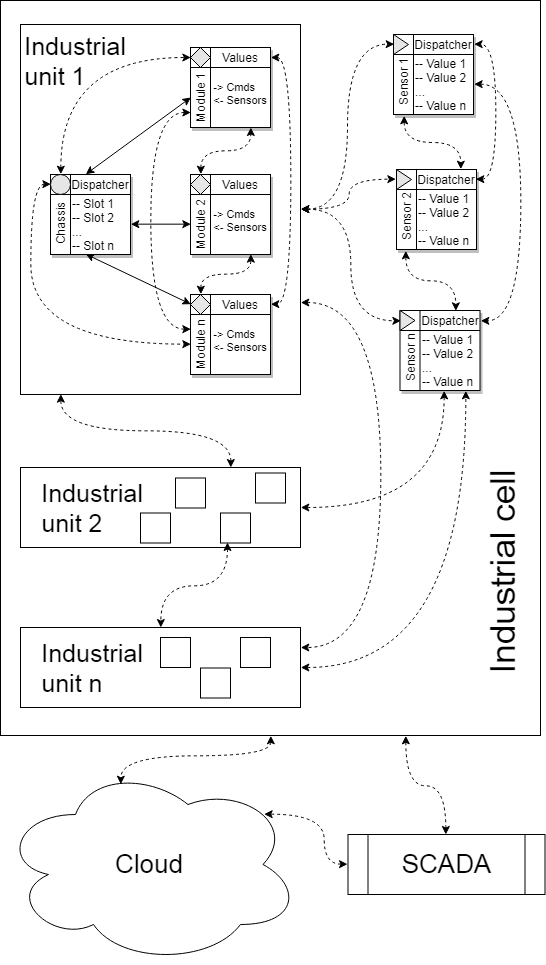
\includegraphics[width=0.5\textwidth]{ch-3/main-arch}
	}
	\caption{Слотовая модель модульного оборудования.}\label{fig:main-arch}
\end{figure}

Слот "--- это запись типа <<ключ-значение>>, из которой диспетчер извлекает необходимые данные. Слот включает в себя следующие поля:

\begin{enumerate}
	\item адрес;
	\item название модуля/датчика;
	\item функции;
	\item возвращаемое значение;
	\item пределы возвращаемого значения.
\end{enumerate}

В качестве адреса выступают IPv6-адрес и порт, необходимые для взаимодействия с модулем. Название должно быть представлено в строковом виде или числовым идентификатором. Доступные для выполнения функции описываются набором G-кодов и М-функций в соответствии со стандартами ISO 6983-1 и ISO/TR 6983-2.
Например, фрезерная головка будет представлять возможность работать с командами M3 и M4 (запуск шпинделя по и против часовой стрелки CW/CCW), M5 (останов шпинделя) и S (скорость вращения); для лазерной головки "--- это будут команды M3 (включить лазер), М5 (выключить) и S (задать мощность в процентах); для магазина инструментов "--- M6 (сменить инструмент) и T (выбрать инструмент из магазина по номеру).  При этом все команды, связанные с перемещением головки в трех основных координатах определяются модулем координатного шасси.

\begin{figure}[ht]
\centerfloat{
	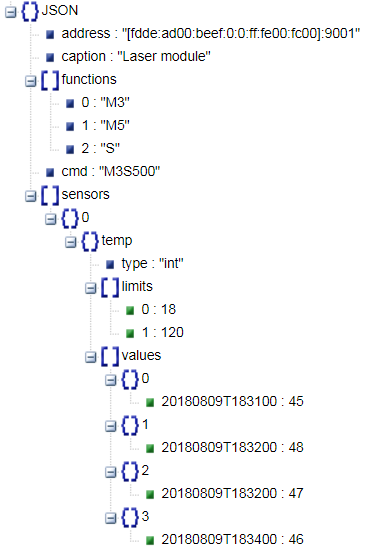
\includegraphics[width=0.3\textwidth]{ch-3/json}
}
\caption{Иерархическая структура единого реестра в формате JSON.}\label{fig:json}
\end{figure}

Возвращаемое значение не обязательно должно быть одним. Описание каждого из них включает в себя тип, пределы и массив значений с временными метками. Диспетчер контролирует выход каждого значения за допустимые пределы, и в случае возникновения такой ситуации – осуществляет анализ возникшей ошибки, и принимается решение о возможности или невозможности продолжения работы оборудования.

Рассмотрим теперь процедуру регистрации модуля в реестре диспетчера. С точки зрения протокола "--- здесь нет никаких проблем: просто передача бинарного JSON-сообщения через очередь сообщений с последующей записью в распределенное хранилище [ссылка]. Однако не стоит забывать, что все диспетчеры и все модули находятся в единой самоорганизующейся mesh-сети. Возникает вопрос "--- как модуль определит к какому конкретно диспетчеру он подключен физически.

Предлагается следующее решение. Физическое подключение каждого модуля реализуется по трехпроводному интерфейсу, где по двум проводникам передается питающее напряжении, а третий используется в качестве линии безопасности (safety line). Линия безопасности объединяет все модули одной единицы оборудования по схеме монтажное И. В данной схеме линия безопасности подтянута резистором к плюсу питания. Так как сопротивление между линией и землей бесконечность, а между питанием и линией равно номиналу резистора, то напряжение на линии равно напряжению питания. То есть высокий уровень или логическая единица. Как уже было сказано выше, все модули подключены к линии и могут замыкать её на землю. Соответственно, на линии будет высокий уровень тогда и только тогда, когда все модули выставят высокий уровень на своих выходах. Как только любой из модулей соединит линию с землей, на ней установится низкий логический уровень и не один модуль не сможет на это повлиять.

\begin{figure}[ht]
\centerfloat{
	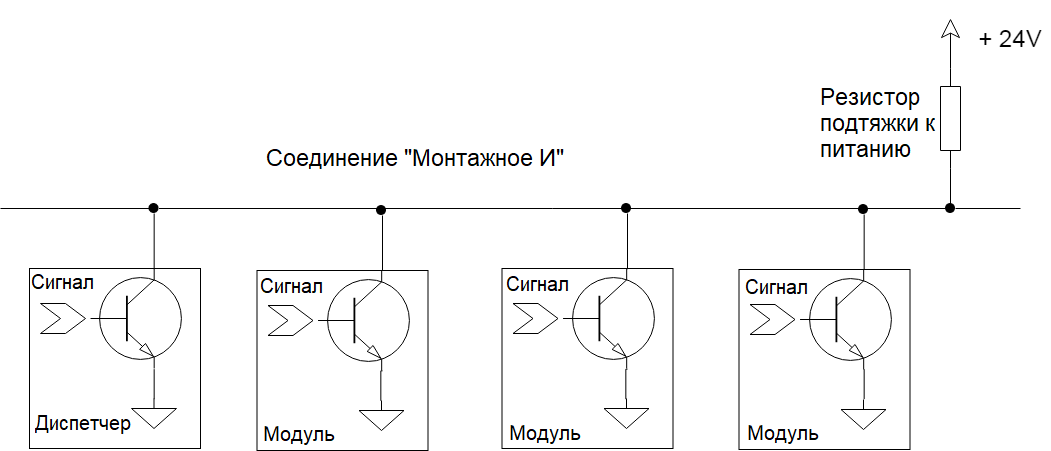
\includegraphics[width=0.7\textwidth]{ch-3/logic-and}
}
\caption{Схема шины безопасности.}\label{fig:logic-and}
\end{figure}

Таким образом, основная задача линии безопасности "--- регистрировать аварийные ситуации. В случае возникновения аварии в любом из модулей, он просто соединяет линию безопасности с землей, что является сигналом для других модулей прекратить работу и перейти в режим восстановления после сбоя. Необходимо отметить, что к этой же линии подключена являющаяся обязательной для любого промышленного оборудования кнопка аварийного останова, а также все двери безопасности, если они предусмотрены конструкцией.

Однако в процессе инициализации модулей линия безопасности может быть использована для регистрации новых модулей. Вновь подключенный модуль вначале осуществляет подключение к сети OpenThread, затем переводит линию безопасности на низкий логический уровень. Диспетчер детектирует это, после чего получает список всех ближайших к нему узлов (neighbors в терминологии OpenThread), выбирает среди них те, которые имеют статус не подключен, после чего просит первого из них перевести линию обратно на высокий логический уровень. Если уровень изменился, значит диспетчер и модуль подключены к одной линии, следовательно, модуль может быть зарегистрирован в реестре. В противном случае, диспетчер переходит к следующему модулю в списке.

При этом нам известно, что все диспетчеры могут общаться между собой, поэтому необходимо установить правило, которое регламентирует порядок инициализации диспетчеров, то есть если один из них проводит наполнение слотов своего реестра, другие должны находится в режиме ожидания и не принимать подключения от модулей. Также понятно, что процесс подключения нового модуля может быть осуществлен только, когда оборудование находится в режиме ожидания.

\section{Выводы по главе 3}

\FloatBarrier